\begin{lstlisting}[caption=Текст программы]
#include <linux/module.h>
#include <linux/kernel.h>
#include <linux/init.h>
#include <linux/fs.h>
#include <linux/time.h>
#include <linux/slab.h>
#include <linux/version.h>

#define wfs_MAGIC_NUMBER 0x13131313
#define SLABNAME "wfs_cache"

MODULE_LICENSE("GPL");
MODULE_AUTHOR("Alexander Stepanov");
MODULE_DESCRIPTION("BMSTU operating systems VFS");

static int size = 7;
module_param(size, int, 0);
static int number = 31;
module_param(number, int, 0);
static int sco = 0;

static void* *line = NULL;

static void co(void* p)
{
    *(int*)p = (int)p;
    sco++;
}

struct kmem_cache *cache = NULL;

static struct wfs_inode
{
     int i_mode;
     unsigned long i_ino;
} wfs_inode;

static struct inode *wfs_make_inode(struct super_block *sb, int mode)
{
    struct inode *ret = new_inode(sb);

    if (ret)
    {
        inode_init_owner(ret, NULL, mode);
        ret->i_size = PAGE_SIZE;
        ret->i_atime = ret->i_mtime = ret->i_ctime = current_time(ret);
        ret->i_private = &wfs_inode;
    }

    return ret;
}

static void wfs_put_super(struct super_block * sb)
{
    printk(KERN_DEBUG "[wfs] super block destroyed!\n");
}

static struct super_operations const wfs_super_ops = {
    .put_super = wfs_put_super,
    .statfs = simple_statfs,
    .drop_inode = generic_delete_inode,
};

static int wfs_fill_sb(struct super_block *sb, void *data, int silent)
{
    struct inode* root = NULL;

    sb->s_blocksize = PAGE_SIZE;
    sb->s_blocksize_bits = PAGE_SHIFT;
    sb->s_magic = wfs_MAGIC_NUMBER;
    sb->s_op = &wfs_super_ops;

    root = wfs_make_inode(sb, S_IFDIR | 0755);
    if (!root)
    {
        printk (KERN_ERR "[wfs] inode allocation failed!\n");
        return -ENOMEM;
    }

    root->i_op   = &simple_dir_inode_operations;
    root->i_fop = &simple_dir_operations;

    sb->s_root = d_make_root(root);
    if (!sb->s_root)
    {
        printk(KERN_ERR "[wfs] root creation failed!\n");
        iput(root);
        return -ENOMEM;
    }

    return 0;
}

static struct dentry* wfs_mount(
    struct file_system_type *type, int flags, char const *dev, void *data
)
{
    struct dentry* const entry = mount_nodev(type, flags, data, wfs_fill_sb);

    if (IS_ERR(entry))
        printk(KERN_ERR "[wfs] mounting failed!\n");
    else
        printk(KERN_DEBUG "[wfs] mounted!\n");

    return entry;
}

static struct file_system_type wfs_type = {
    .owner = THIS_MODULE,
    .name = "wfs",
    .mount = wfs_mount,
    .kill_sb = kill_litter_super,
};

static int __init wfs_init(void)
{
    int i;
    int ret;

    if (size < 0)
    {
        printk(KERN_ERR "[wfs] invalid argument\n");
        return -EINVAL;
    }

    line = kmalloc(sizeof(void*) * number, GFP_KERNEL);

    if (line == NULL)
    {
        printk(KERN_ERR "[wfs] kmalloc error\n" );
        kfree(line);
        return -ENOMEM;
    }

    for (i = 0; i < number; i++)
    {
        line[i] = NULL;
    }

    cache = kmem_cache_create(SLABNAME, size, 0, SLAB_HWCACHE_ALIGN, co);

    if (cache == NULL)
    {
        printk(KERN_ERR "[wfs] kmem_cache_create error\n" );
        kmem_cache_destroy(cache);
        kfree(line);
        return -ENOMEM;
    }

    for (i = 0; i < number; i++)
    {
        if (NULL == (line[i] = kmem_cache_alloc(cache, GFP_KERNEL))) {
            printk(KERN_ERR "[wfs] kmem_cache_alloc error\n");

            for (i = 0; i < number; i++)
            {
                kmem_cache_free(cache, line[i]);
            }

            kmem_cache_destroy(cache);
            kfree(line);
            return -ENOMEM;
        }
    }

    printk(KERN_INFO "[wfs] allocate %d objects into slab: %s\n",
        number, SLABNAME);
    printk(KERN_INFO "[wfs] object size %d bytes, full size %ld bytes\n",
        size, (long)size * number);
    printk(KERN_INFO "[wfs] constructor called %d times\n", sco);

    ret = register_filesystem(&wfs_type);

    if (ret!= 0)
    {
        printk(KERN_ERR "[wfs] module cannot register filesystem!\n");
        return ret;
    }

    printk(KERN_DEBUG "[wfs] module loaded!\n");
    return 0;
}

static void __exit wfs_exit(void)
{
    int i;
    int ret;

    for (i = 0; i < number; i++)
        kmem_cache_free(cache, line[i]);

    kmem_cache_destroy(cache);
    kfree(line);

    ret = unregister_filesystem(&wfs_type);

    if (ret!= 0)
        printk(KERN_ERR "[wfs] module cannot unregister filesystem!\n");

    printk(KERN_DEBUG "[wfs] module unloaded!\n");
}

module_init(wfs_init);
module_exit(wfs_exit);
\end{lstlisting}

\begin{figure}[H]
    \centering
    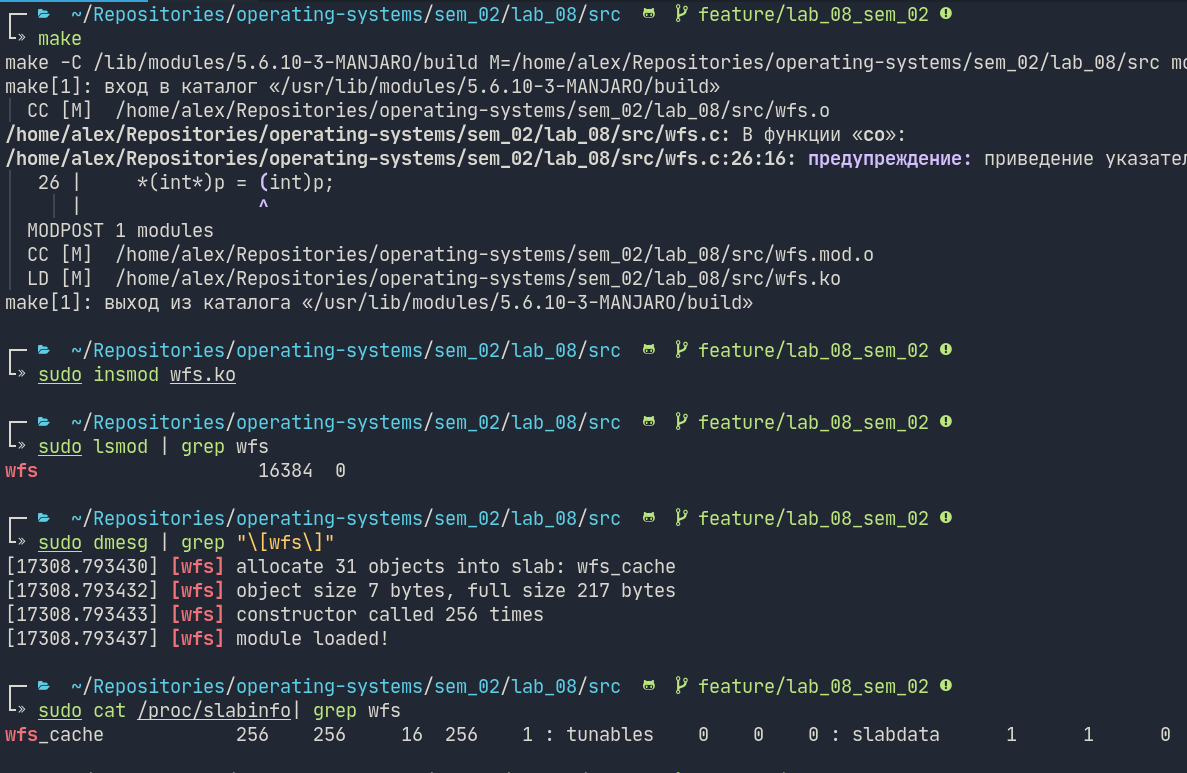
\includegraphics[scale=0.4]{img/insmod.png}
    \caption{Загрузка модуля}
\end{figure}

\begin{figure}[H]
    \centering
    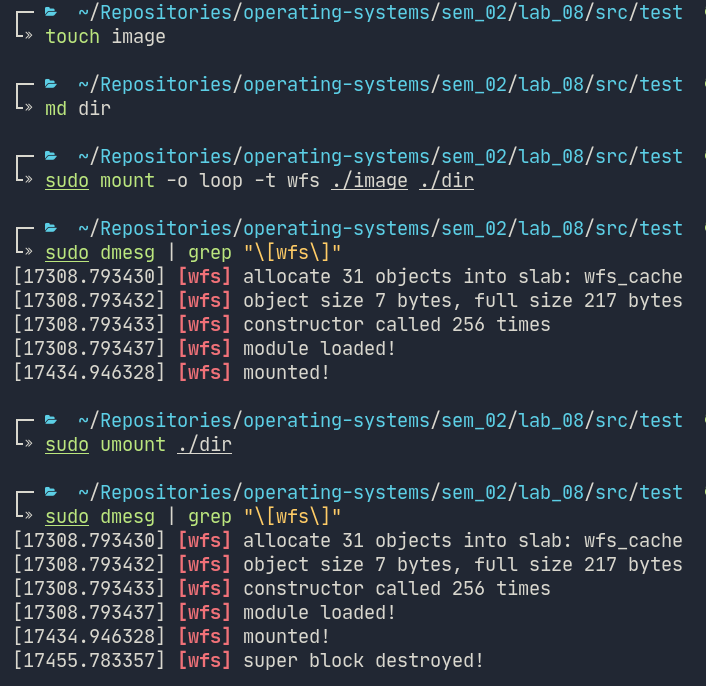
\includegraphics[scale=0.45]{img/mount.png}
    \caption{Монтирование файловой системы}
\end{figure}

\begin{figure}[H]
    \centering
    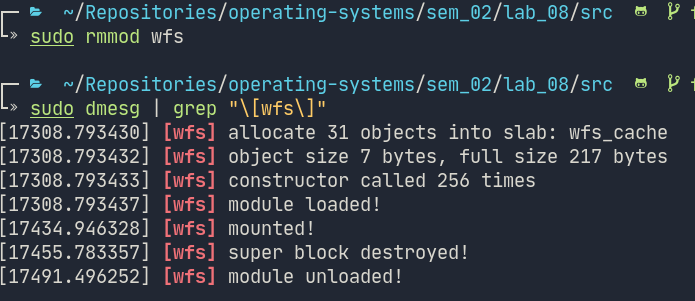
\includegraphics[scale=0.6]{img/unload.png}
    \caption{Выгрузка модуля}
\end{figure}

\begin{figure}[H]
    \centering
    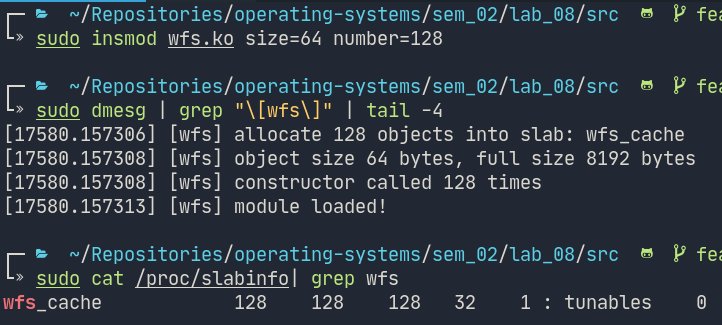
\includegraphics[scale=0.6]{img/parameters.png}
    \caption{Загрузка модуля с заданием параметров}
\end{figure}
